% !TEX root = main.tex
\chapter*{Acknowledgements}

We would like to thank our supervisors Jens Honore Walther and Robert Flemming Mikkelsen, for giving us the opportunity to learn intricate details about our own personal project. A special thanks to everyone on the team of Vermilion Racing, who in less than a year managed to make a dream reality. Vermilion Racing is going to compete at the Silverstone race track the 10\textsuperscript{th} of July, where all of our ideas and designs are going to be tested to the limit.

The sponsors who made this project possible are all found on the following page. A big thanks goes out to everyone who supported us and assisted us in creating this project.

Thanks to Rasmus Himborg and Philips Lighting Denmark, for helping us machine a 1/4 scale wing used in the wind tunnel tests.

Thanks to Daniel Rasmussen, Bo Tranberg and Jacob Buch for assisting with graphical layout of the report.

Thanks to Nicolai Boertmann and Daniel Rasmussen for the help building the composite wings.

Thanks to DTU Skylab, and especially Martin Meister, Rasmus Bruun, Ralle Malone and Tonja Kramer for always having the time to help us when things looked most dire.

Lastly, a thank to Nenad Mijatovic. Nenad is the overall supervisor for Vermilion Racing and is a significant reason we recently became a DTU Blue Dot project - a highly prestigious title that will ensure that the team will survive for many years to come.

\begin{figure}
  \makebox[\textwidth][c]{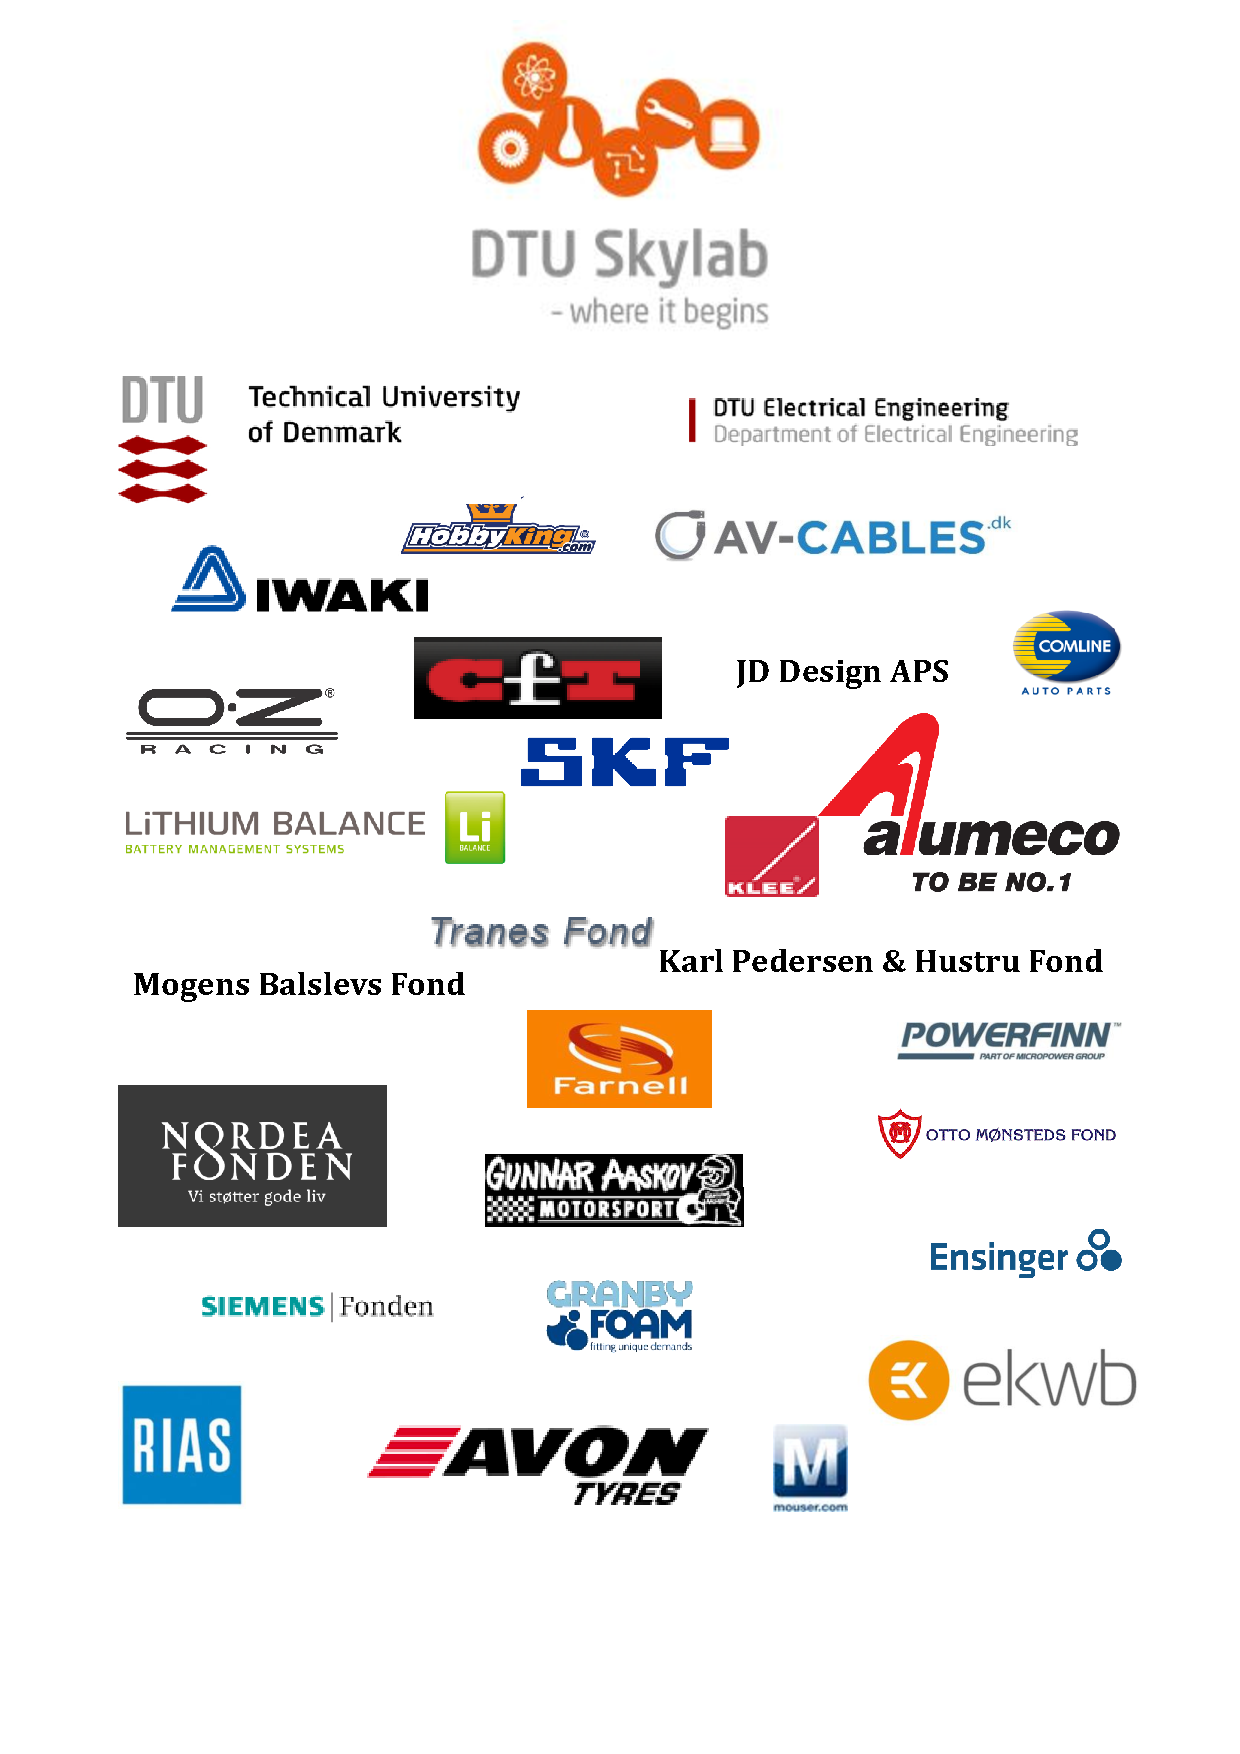
\includegraphics[width=1.5\textwidth]{sponsorstack}}
  \label{fig:sponsorstack}
\end{figure}
